\chapter{Resultados}

\section{Experimentación}
\comentarioM{Breve introducción de la experimentación en general (explicar subsecciones y cosas generales)}


\comentarioM{Comentar brevemente la evaluación del tracking y eleccion de parametros y explicar por que se eligio usar como deteccion el valor sacado del ground truth.}

Para cuantificar la efectividad y robustes del tracking del algoritmo elegido decidimos evaluar las siguientes variables:
\begin{itemize}
	\item Taza de falsos positivos: cantidad de veces que el algoritmo reporta haber encontrado el objeto cuando en realidad no está en la imagen
	\item Taza de falsos negativos: cantidad de veces que el algoritmo no encuentra el objeto cuando en realidad el mismo está en la imagen
	\item Promedio de área solapada: promedio de solapamiento de área\footnote{Ver http://pascallin.ecs.soton.ac.uk/challenges/VOC/voc2011/workshop/voc\_seg.pdf, página 7, Evaluation Metric} entre el objeto reportado por el algoritmo y el ground truth durante toda la escena
	\item Desviación estándar del área solapada
	\item Porcentaje de veces seguido: de todas las veces que el objeto aparece en la escena obtenemos el porcentaje de veces que el algoritmo de seguimiento fue exitoso	
\end{itemize}

\subsection{Elección de parámetros RGB}
\comentarioM{No se donde explicar esto ni donde explicar todos los métodos que probé y que fui descartando con pruebas mas sencillas.}
EL método de seguimiento por comparación de histogramas explicado en la sección \comentarioM{SECCION DONDE SE EXPLICA LA COMPARACION DE HISTOGRAMAS} es un método sencillo pero que posee muchas variables para explorar que permiten modificar la eficacia del algoritmo. Decidimos reducir el número de variables a explorar variando únicamente el método de comparación de histogramas, el modelo de color elegido para comparar (RGB o HSV), un umbral para la comparación entre el objeto en el frame actual y el objeto encontrado en el frame anterior y otro para comparar el objeto en el frame actual y el modelo del objeto buscado.

\subsection{Evaluación del tracking RGB}
A continuación se muestran los resultados del algoritmo de seguimiento elegido para las imágenes RGB con los valores de los parámetros ya fijados. Para todas las pruebas se eligieron tres objetos distintos que aparecen en dos escenas, todos sacados de la base de datos indicada en la sección \ref{base_rgbd}.

\begin{table}[h]
    \begin{tabular}{|c|c|c|c|c|c|}
    \hline
    & \multirow{2}{2.4cm}{\% promedio de overlap} & & \multirow{2}{2cm}{\% veces seguido} & \multirow{2}{1.6cm}{Falsos Positivos} & \multirow{2}{1.6cm}{Falsos Negativos}\\
	Objeto & & overlap STD & & &\\
    \hline
    Taza   & 36.75      & 26.20       & 90.79             & 0                & 0\\
    \hline
    Gorra  & 57.93      & 21.77       & 80.49             & 0                & 0\\
    \hline
    Bowl   & 74.13      & 40.24       & 30.91             & 0                & 0\\
    \hline
    \end{tabular}
\caption{Resultados del tracking RGB utilizando como detección los valores sacados de la base de datos}
\label{tabla_rgb}
\end{table}

Como podemos ver en la tabla \ref{tabla_rgb} el tracking se comporta de manera muy diversa dependiendo del objeto que se esté analizando. En los casos de la taza y la gorra el algoritmo es exitoso en la mayoría de los casos, 90\% y 80\% respectivamente. De todas maneras si se observa el promedio de solapamiento vemos que se comporta mucho mejor en el caso de la gorra. Creemos que esto se debe a la marcada diferencia de color entre la gorra y el fondo de la imagen. Esto no sucede en el caso de la taza en el que repetidas veces el color de fondo varía entre colores y tonos similares a los de esta lo que provoca que la comparación de histogramas no sea robusta. En el caso del bowl el promedio de solapamiento es alto pero se debe a que el porcentaje de veces que se siguió al objeto es bajo. Como el algoritmo de detección es el ideal, cuantas más veces se usa la detección mejor es el porcentaje de solapamiento. Este análisis está hecho en una escena distinta a la escena de la taza y la gorra. Notamos que en esta escena los cambios en la luminosidad y la coloración son muy notorios lo que afecta negativamente al algoritmo.


\begin{figure}
	\centering
	\begin{subfigure}[b]{\textwidth}
		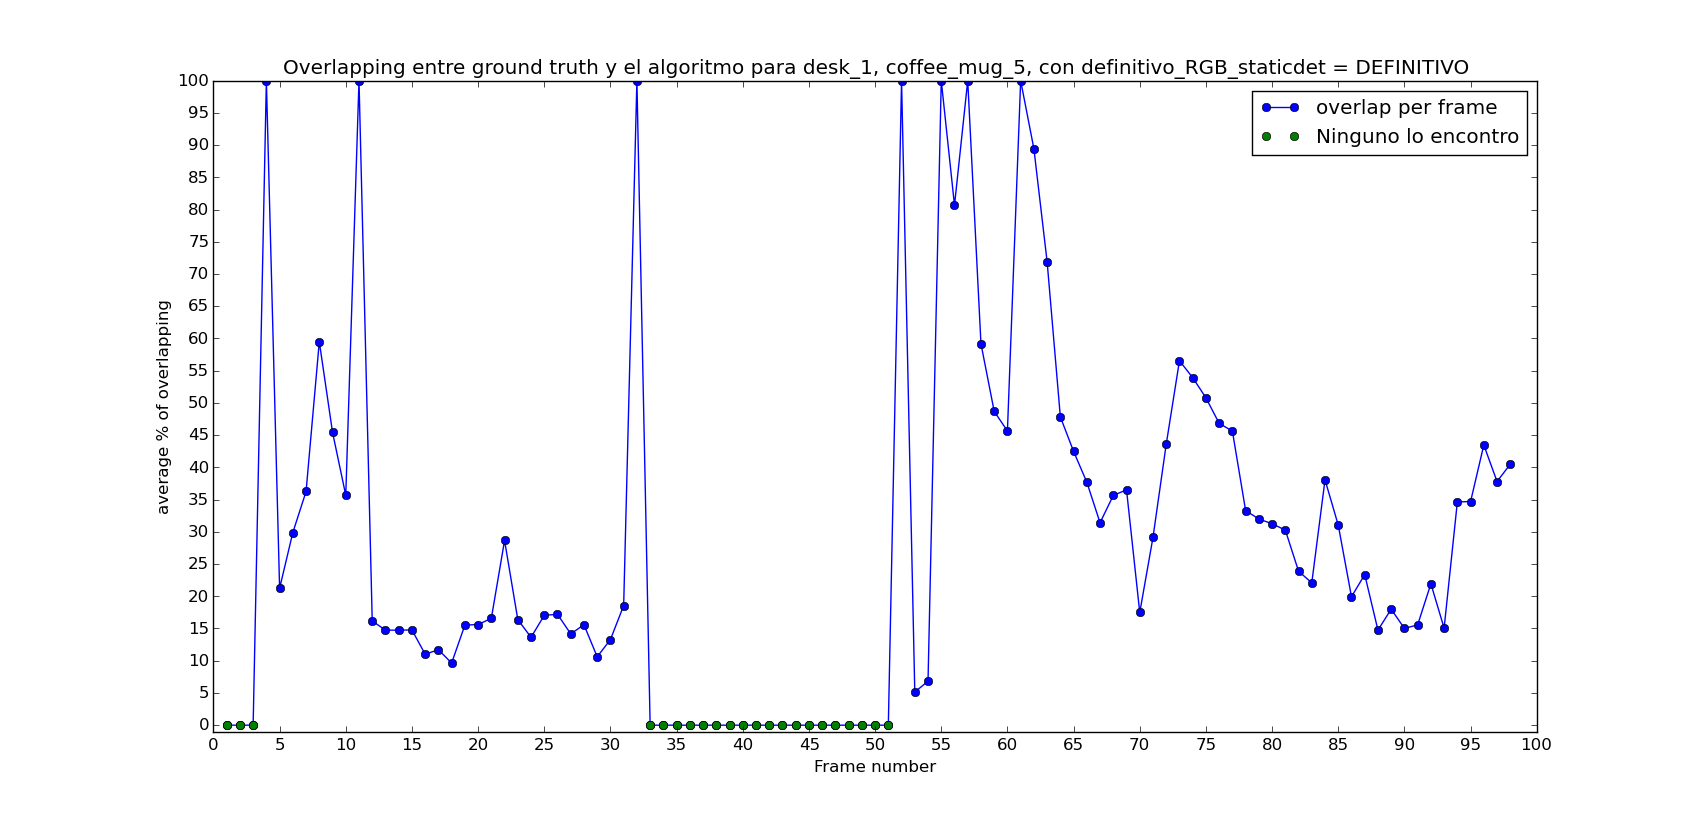
\includegraphics[width=\textwidth]{img/seguimientoframeaframe-rgb-taza.png}
		\caption{Seguimiento frame a frame para la taza}
		\label{frame_frame_taza}
	\end{subfigure}
	\quad
	\begin{subfigure}[b]{\textwidth}
		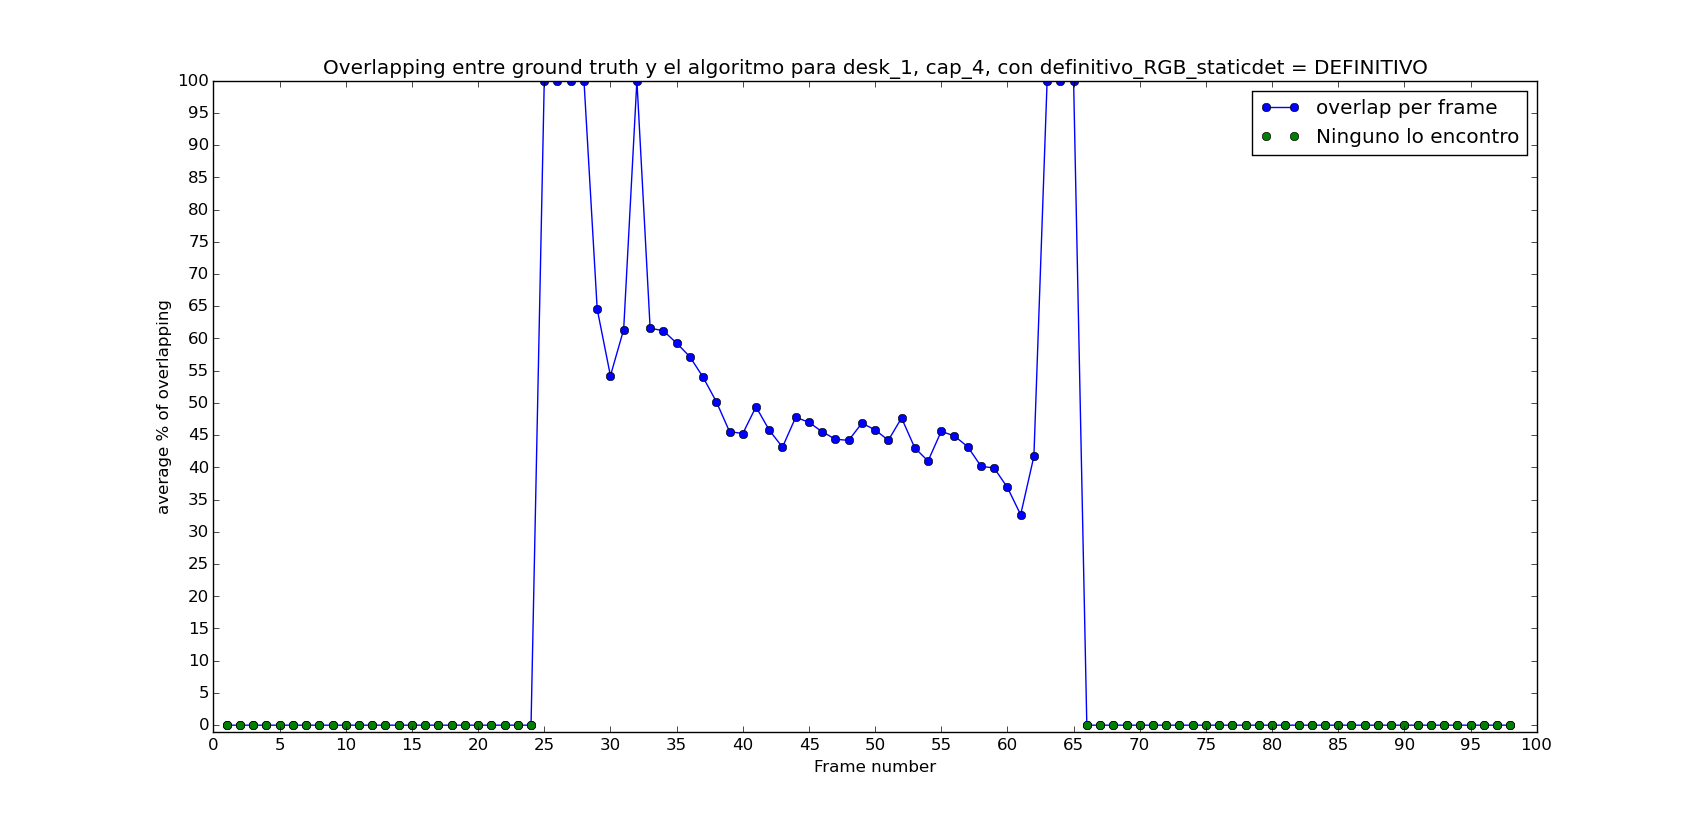
\includegraphics[width=\textwidth]{img/seguimientoframeaframe-rgb-gorra.png}
		\caption{Seguimiento frame a frame para la gorra}
		\label{frame_frame_gorra}
	\end{subfigure}	
	\quad
	\begin{subfigure}[b]{\textwidth}
		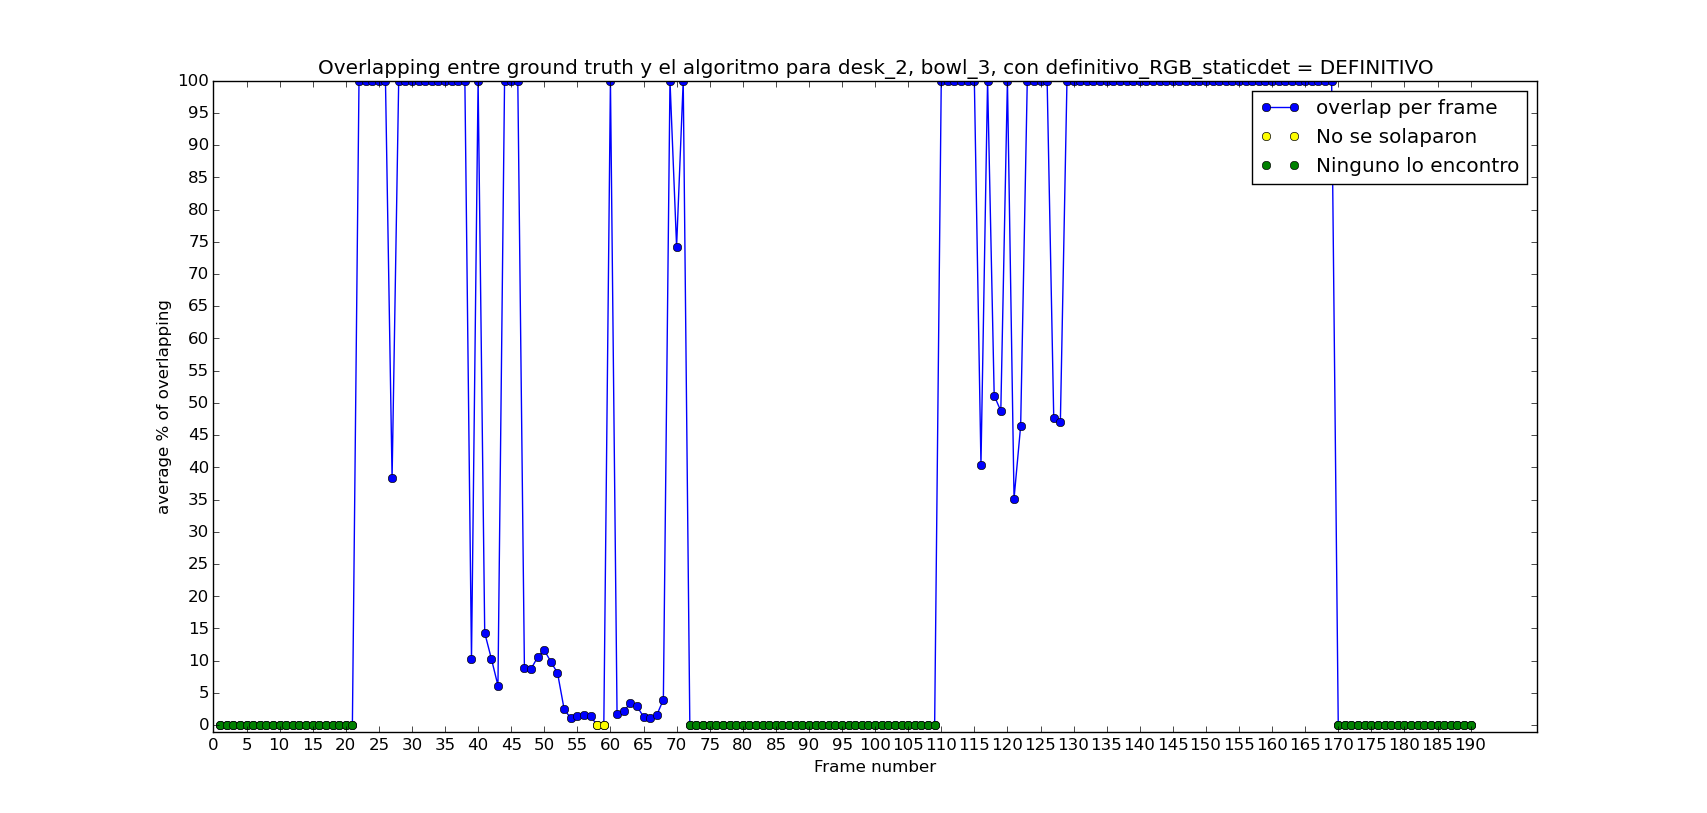
\includegraphics[width=\textwidth]{img/seguimientoframeaframe-rgb-bowl.png}
		\caption{Seguimiento frame a frame para el bowl}
		\label{frame_frame_bowl}
	\end{subfigure}
	\caption{\comentarioM{Descripcion}}
	\label{frame_frame}
\end{figure}

En la figura \ref{frame_frame} se intenta visualizar mejor el comportamiento del algoritmo para cada objeto en las distintas escenas. En cada gráfico se muestra para cada escena y por cada frame el porcentaje de solapamiento entre el área del objeto reportada por el algoritmo y la indicada por el ground truth. Los puntos que están en 0 de color verde indican que el objeto no fue encontrado y que eso coincide con el ground truth, como es el caso de los gráficos \ref{frame_frame_taza} y \ref{frame_frame_gorra}. En el gráfico \ref{frame_frame_bowl} se ven dos puntos en 0 de color amarillo. Esto indica que el algoritmo reporta haber seguido al objeto pero que el área no se solapa con el área del ground truth. Para los tres gráficos, todas los frames cuyo área es igual a 100\% se corresponde con las veces que el algoritmo de detección fue corrido, es decir, cuando falló el seguimiento. 

Se puede ver en el gráfico \ref{frame_frame_taza} que el algoritmo de seguimiento reporta un área que se solapa entre un 15\% y un 50\% en la mayoría de los casos. En el gráfico \ref{frame_frame_gorra} la mayoría oscila entre un 35\% y un 50\% y en el gráfico \ref{frame_frame_bowl} se observa que la mayoría se encuentra entre un 1\% y un 10\%. Una hipótesis es que el algoritmo no funciona correctamente cuando los objetos tienen poca textura y esto empeora si existen objetos cercanos cuya textura sea similar a la del objeto que se está buscando. Este sería el caso de la taza y del bowl. Ambos son objetos con poca textura de color blanco que pueden camuflarse con otros objetos de la escena. \comentarioM{No estaría bueno indicar el porcentaje de solapamiento promedio del algoritmo de seguimiento sin tener en cuenta las detecciones????}


\section{Discusión}